
\Chainmail assertions (details in appendix \ref{sect:standard}) consist of (pure) expressions \e, comparisons between expressions, classical
assertions about the contents of heap and stack, the usual logical
connectives, as well as our holistic concepts.
In this section we focus on the novel,
 holistic, features of \Chainmail (permission, control, time, space, and viewpoint),
as well as our wish to support some form of recursion while keeping the logic of assertions classical.
% SD I removed the belowas it is no longer true here. % don't understand what you mean so i have deleted the next paragraph
%\sdN{Expressions include variables, field lookup, and the execution of (pure) ghost methods. 
%This  supports recursion at the level of expressions; therefore, the value of  an expression  may be
% undefined (either because of infinite recursion, or because the expression accessed undefined fields or variables). 
 %Assertions of the form   $\e$=$\e'$ are satisfied only if both $\e$ and $\e'$ are defined. Because we do not support 
% recursion at the level of assertions, assertions form a classical logic (\eg $\A \vee \neg\A$ is a tautology)
%}
%Assertions support the comparison of expressions, and the usual logical connectives
%(Appendix, section \ref{sect:standard}), as well as the usual connectives discussed below.
%We now define the syntax and semantics of expressions and holistic assertions.
%\sd{The novel, holistic, features of \Chainmail (permission, control, time, space, and viewpoint),
%as well as our wish to support some form of recursion while keeping the logic of assertions classical,  introduced 
%challenges, which we discuss in this section.}

\subsection{Syntax of Assertions}
 
We now define the syntax and semantics of expressions and holistic assertions.
\sd{The novel, holistic, features of \Chainmail (permission, control, time, space, and viewpoint),
as well as our wish to support some form of recursion while keeping the logic of assertions classical,  introduced 
challenges, which we discuss in this section.}

 \subsection{Syntax of Assertions}
 


\begin{definition}[Assertions]  \sd{Assertions consist of (pure) expressions \e, classical assertions about the contents of heap/stack, the usual logical  connectives, as well as our holistic concepts.}
\label{def:assertions}


 $\begin{array}{lcl}
  ~  \\
 \SE  &\BBC&    \kwN{true}   ~\SOR~  \kwN{false}   ~\SOR~  \kwN{null}  ~\SOR~  \x  \   ~\SOR~  
     \   \SE=\SE    ~\SOR~ \kwN{if}\, \SE\,   \kwN{then}\,  \SE\,    \kwN{else}\, \SE    ~\SOR~  \SE.\f\lp\ \SE^* \ \rp\\
     \\
 \A &\ \BBC   &   \SE \   \mid \  \SE=\SE  \mid \   \SE:\prg{ClassId}  \ \mid \
    \SE\in\prg{S}   \mid  \  \\
    &
  &  \A \rightarrow \A  \ \mid\  \     \A \wedge \A  \ \mid\  \  \A \vee \A  \ \mid\  \ \neg A   \ \mid \ \\
  & &  \forall \x.\A  \ \mid \  \forall \prg{S}:SET.\A  \ \mid  \  \exists \x.\A  \ \mid \  \exists \prg{S}:SET.\A  \  \ \mid\   \\
 &    &  \CanAccess x y %\ \mid\  \ \Changes e 
           \ \mid\  \Calls {\prg{x}}  {\prg{m}} {\prg{x}}  {\prg{x}^*}\\          
% &    &  \kjx{\CanAccess x y \ \mid\  \ \Changes e 
%           \ \mid\  \Calls {\prg{x}}  {\prg{m}} {\prg{x}}  {\prg{x}^*} }\\
&    &  \Next \A  \ \mid \   \Future \A \ \mid \  \Prev \A   \ \mid \ \Past \A \ \mid \\  
 &    &        \Using \SF  \A  \ \mid \  \External \x     \\
% &    &   \kjx{\Using \SF  \A  \ \mid \  \External \x \ \mid \ \prg{x} \obeys \prg{S} }  \\
 \\
 \x, \f, \m &\BBC&  \prg{Identifier}  ~ \\
\end{array}$
\end{definition}
%% \footnote{
%% The operators $\wedge$, $\vee$,  $\neg$ and $\forall$  could have been
%% defined  through the usual shorthands, \eg, $\neg \A$ is short for
%% $\A \rightarrow \ff$ \etc, but here we give full definitions
%% instead\kjx{can we just cut this please?}}

\jm{
\begin{definition}[Assertions]  \sd{Assertions consist of (pure) expressions \e, classical assertions about the contents of heap/stack, the usual logical  connectives, as well as our holistic concepts.}
\label{def:assertions}


 $\begin{array}{lcl}
  ~  \\
 \prg{v}  &\BBC&    \kwN{true}   ~\SOR~  \kwN{false}   ~\SOR~  \kwN{null}  ~\SOR~  \alpha  \\
  ~  \\
 \SE  &\BBC&    \prg{v}\ ~\SOR~ \SE=\SE    ~\SOR~ \kwN{if}\, \SE\,   \kwN{then}\,  \SE\,    \kwN{else}\, \SE    ~\SOR~  \SE.\f\lp\ \SE^* \ \rp\\
     \\
 \A &\ \BBC   &   \SE \   \mid \  \SE=\SE  \mid \   \SE:\prg{ClassId}  \ \mid \
    \SE\in\prg{S}   \mid  \  \\
    &
  &  \A \rightarrow \A  \ \mid\  \     \A \wedge \A  \ \mid\  \  \A \vee \A  \ \mid\  \ \neg A   \ \mid \ \\
  & &  \forall \alpha.\A  \ \mid \  \forall \prg{S}:SET.\A  \ \mid  \  \exists \alpha.\A  \ \mid \  \exists \prg{S}:SET.\A  \  \ \mid\ \forall \m.\A \ \mid\ \exists \m. \A \\
 &    &  \CanAccess {\alpha_1} {\alpha_2} %\ \mid\  \ \Changes e 
           \ \mid\  \Calls {\alpha_1}  {\prg{m}} {\alpha_2}  {\prg{v}^*}\\          
% &    &  \kjx{\CanAccess x y \ \mid\  \ \Changes e 
%           \ \mid\  \Calls {\prg{x}}  {\prg{m}} {\prg{x}}  {\prg{x}^*} }\\
&    &  \Next \A  \ \mid \   \Future \A \ \mid \  \Prev \A   \ \mid \ \Past \A \ \mid \\  
 &    &        \Using \SF  \A  \ \mid \  \External \alpha  \jm{\ \mid\ \prg{name}\langle \alpha, \x \rangle } \\
% &    &   \kjx{\Using \SF  \A  \ \mid \  \External \x \ \mid \ \prg{x} \obeys \prg{S} }  \\
 \\
 \x, \f, \m &\BBC&  \prg{Identifier}  ~ \\
\end{array}$
\end{definition}}
 
Expressions support calls with parameters  ($\e.\f(\e^*)$); these are calls to ghostfield
functions. This  supports recursion at the level of expressions; therefore, the value of  an expression  may be
undefined (either because of infinite recursion, or because the expression accessed undefined fields or variables). 
Assertions of the form   $\e$=$\e'$ are satisfied only if both $\e$ and $\e'$ are defined. Because we do not support 
recursion at the level of assertions, assertions from a classical logic (\eg $\A \vee \neg\A$ is a tautology).
 
We will discuss evaluation of expressions in section \ref{sect:expressions}, standard assertions about heap/stack and logical
 connectives in \ref{sect:standard}. 
 \sophia{We have discussed  the treatment of  permission, control, space, and viewpoint  in 
the main text in the  Definitions 3-7  in section \ref{sect:pcsv} %HARD
the treatment of time in  Definitions 8,9 in the main text, section \ref{sect:time},
We will discuss properties of assertions in Lemmas \ref{lemma:classic}-\ref{lemma:classic:two}.}
 The judgement $\M\mkpair \M', \sigma  \models \A$ expresses that $\A$ holds in  $\M\mkpair \M'$ and $\sigma$, and 
while $\M\mkpair \M', \sigma  \not\models \A$  expresses that $\A$ does not hold  in  $\M\mkpair \M'$ and $\sigma$.
 
\subsection{Values of Expressions}
\label{sect:expressions}

The value  of  an expression  is described through judgment $ \M,\, \sigma, \SE \ \hookrightarrow\  v$,
defined in  Figure \ref{fig:ValueSimpleExpressions}.
We use the configuration, $\sigma$, to read the contents of the top stack frame
% value of variables defined in the stack frame
(rule ${\sf {Var\_Val}}$) or the contents of the heap (rule
${\sf {Field\_Heap\_Val}}$). We use the module, \M, to find the  ghost field declaration corresponding to the
ghost field being used. 


The treatment of fields and ghost fields is described in rules ${\sf {Field\_Heap\_Val}}$,\\  ${\sf {Field\_Ghost\_Val}}$ and 
${\sf {Field\_Ghost\_Val2}}$.  If the field \f~ exists in the heap, then its value is returned (${\sf {Field\_Heap\_Val}}$). 
Ghost field reads, on the other hand, have the form $\e_0.\f(\e_1,...\e_n)$, and their value is
described in rule ${\sf {Field\_Ghost\_Val}}$:
%
The lookup function $\mathcal G$  (defined in the obvious way in the Appendix, Def.\ref{def:lookup})
returns the expression constituting the body for that ghost field, as defined in the class of $\e_0$.
We return  that expression
evaluated in a configuration where the formal parameters have been substituted by the values of the actual
parameters.

Ghost fields support recursive definitions. For example, imagine a module $\M_0$ with
a class \prg{Node} which has a field called \prg{next}, and which 
had a ghost field \prg{last}, which finds  the last \prg{Node} in a sequence
and is defined recursively as \\
$~ \strut \hspace{.1cm}$ \ \ \ \prg{if}\ \ \prg{this.next}=\prg{null}\  \prg{then} \ \prg{this} \ \prg{else} \ \prg{this.next.last},\\
and another ghost field \prg{acyclic}, which expresses that a sequence is acyclic,
defined recursively as \\
$~ \strut \hspace{.1cm}$ \ \ \ \prg{if}\ \ \prg{this.next}=\prg{null}\  \prg{then} \ \prg{true} \ \prg{else} \ \prg{this.next.acyclic}.

The relation $ \hookrightarrow$ is partial. 
For example, assume   a configuration
$\sigma_0$ where
\prg{acyc} points to a \prg{Node} whose field \prg{next} has value \prg{null}, and   
\prg{cyc} points to a \prg{Node} whose field \prg{next} has the same value as \prg{cyc}. Then,   
$\M_0,\sigma_0,\,\prg{acyc.acyclic}  \ \hookrightarrow\  \prg{true}$, but we would have no value for 
$\M_0,\sigma_0,\, \prg{cyc.last}  \ \hookrightarrow\  ...$, nor for
$\M_0,\sigma_0,\, \prg{cyc.acyclic}  \ \hookrightarrow\  ...$.

Notice also that for an expression of the form  
\prg{\e.\f}, both ${\sf {Field\_Heap\_Val}}$ and ${\sf {Field\_Ghost\_Val2}}$ could be applicable: rule ${\sf {Field\_Heap\_Val}}$
will be applied if \prg{f} is a field of the object at \prg{e}, while rule ${\sf {Field\_Ghost\_Val}}$
will be applied if \prg{f} is a ghost field of the object at \prg{e}. We expect the set of fields and ghost fields in a 
given class to be disjoint.
This allows a specification to be agnostic over whether a field is a physical field or just ghost information.
For example, assertions (1) and (2) from  section  \ref{sect:motivate:Bank}
 talk about the \prg{balance} of an \prg{Account}. 
In module $\M_{BA1}$ (Appendix~\ref{Bank:appendix}), where we keep the balances in the account objects, this is a physical field. 
In $\M_{BA2}$ (also in Appendix~\ref{Bank:appendix}), where we keep the
balances in a ledger, this is ghost information.  
 


\begin{figure*}
{$\begin{array}{l}
\begin{array}{llll}
\inferenceruleN {True\_Val} {
}
{
 \M,\, \sigma, \kwN{true} \ \hookrightarrow\  \kwN{true}
}
& 
\inferenceruleN {False\_Val} {
}
{
 \M,\, \sigma, \kwN{false} \ \hookrightarrow\  \kwN{false}
}
&
\inferenceruleN  {Null\_Val} {
}
{
 \M,\, \sigma, \kwN{null} \ \hookrightarrow\  \kwN{null}
}
&
\inferenceruleN {Var\_Val} {
}
{
 \M,\,  \sigma, \x \ \hookrightarrow\   \sigma({\x})
}
\end{array}
\\ \\
\begin{array}{lll}
\begin{array}{l}
\inferenceruleNM{Field\_Heap\_Val} {
 \M,\,  \sigma, \SE \ \hookrightarrow\   \alpha \hspace{1.5cm} 
 \sigma(\alpha,\f)=v
}
{
 \M,\, \sigma, \SE.\f  \ \hookrightarrow\   v
}
\\
\\
\inferenceruleNM{Field\_Ghost\_Val2} {
 \M,\, \sigma, \SE.\f \lp \rp \ \hookrightarrow\   v
}
{
 \M,\, \sigma, \SE.\f   \ \hookrightarrow\   v
}
\end{array}
& &
\inferenceruleNM{Field\_Ghost\_Val}
{
~ \\
 \M,\, \sigma, \SE_0   \ \hookrightarrow\  \alpha
\\
 \M,\, \sigma, \SE_i  \ \hookrightarrow\   v_i\ \ \ \ i\in\{1..n\}
 \\
{\mathcal{G}}
(\M, {\ClassOf {\alpha} {\sigma}}, {\f}) \  =  
\ \f\lp \p_1, \ldots \p_n \rp \lb\ \SE \ \rb
  \\
  \M,\,\sigma[\p_1\mapsto v_1, .... \p_n\mapsto v_n], \SE    \hookrightarrow_{\SAF}\   v 
 }
{
 \M,\,  \sigma, \ \SE_0.\f \lp \SE_1,....\SE_n\rp \hookrightarrow   \ v
}
\\ \\
\inferenceruleNM{If\_True\_Val} 
{
 \M,\,  \sigma, \SE \ \hookrightarrow\   \prg{true}  \\
   \M,\,  \sigma, \SE_1 \ \hookrightarrow\   v  
}
{
 \M,\, \sigma, \kwN{if}\ \SE\  \kwN{then} \ \SE_1 \ \kwN{else} \ \SE_2\  \hookrightarrow  \ v
}
& &
\inferenceruleNM {If\_False\_Val} 
{
 \M,\,  \sigma, \SE \ \hookrightarrow\   \prg{false}  \\
   \M,\,  \sigma, \SE_2 \ \hookrightarrow\   v  }
{
 \M,\, \sigma, \kwN{if}\ \SE\  \kwN{then} \ \SE_1 \ \kwN{else} \ \SE_2\  \hookrightarrow\  v
}
\\ \\ 
\inferenceruleNM {Equals\_True\_Val} 
{
 \M,\,  \sigma, \SE_1 \ \hookrightarrow\    v \\
   \M,\,  \sigma, \SE_2 \ \hookrightarrow\     v 
}
{
 \M,\, \sigma, \SE_1 =  \SE_2 \hookrightarrow \prg{true}
}
& &
\inferenceruleNM {Equals\_False\_Val} 
{
 \M,\,  \sigma, \SE_1 \ \hookrightarrow\    v \\
   \M,\,  \sigma, \SE_2 \ \hookrightarrow\     v' \hspace{2cm}  v\neq v'
}
{
 \M,\, \sigma, \SE_1 =  \SE_2 \hookrightarrow \ \prg{false}
}
\end{array}
\end{array}
$}
\caption{Value of  Expressions}
\label{fig:ValueSimpleExpressions}
\end{figure*}

\subsection{Satisfaction of Assertions - standard}
\label{sect:standard}
\sd{
We now define the semantics of assertions involving expressions, the heap/stack, and logical connectives.
The semantics are unsurprising, except, perhaps the relation between validity of assertions and the values of
expressions.
}


 \begin{definition}[Interpretations for simple expressions]

For a runtime configuration, $\sigma$,    variables $\x$ or \SF, we define its interpretation as follows:

\begin{itemize}
  \item
  $\interp {\x}{\sigma}$ $ \triangleq$ $\phi(\x)$  \ \ if \ \ $\sigma$=$(\phi\cdot\_,\_)$
  \item
  $\interp {\SF}{\sigma}$ $ \triangleq$ $\phi(\SF)$  \ \ if \ \ $\sigma$=$(\phi\cdot\_,\_)$
  \item
    $\interp {\x.\f}{\sigma}$ $ \triangleq$ $\chi(\interp {\x}{\sigma},\f)$  \ \ if \ \ $\sigma$=$(\_,\chi)$
   \end{itemize}
\end{definition}   

 
\begin{definition}[ Basic Assertions] For modules $\M$, $\M'$,  configuration $\sigma$,  we define$:$
%validity of basic assertions: 
\label{def:valid:assertion:basic}
\begin{itemize}
\item
$\M\mkpair \M', \sigma \models\SE$ \IFF   $ \M,\,  \sigma, \SE \ \hookrightarrow\   \prg{true}$ 
\item
$\M\mkpair \M', \sigma \models\SE=\SEPrime$ \IFF there exists a value $v$ such that  $\M,\,  \sigma, \SE \ \hookrightarrow\   v$  and $ \M,\,  \sigma, \SEPrime \ \hookrightarrow\   v$.
           \item
$\M\mkpair \M', \sigma \models\SE:\prg{ClassId}$ \IFF there exists an address $\alpha$ such that \\
$\strut ~ $ \hspace{2in} \hfill   
 $ \M,\,  \sigma, \SE \ \hookrightarrow\   \alpha$, and $\ClassOf{\alpha}{\sigma}$ = \prg{ClassId}.
\item
$\M\mkpair \M', \sigma \models \SE\in \prg{S}$ \IFF there exists a value $v$ such that 
 $ \M,\,  \sigma, \SE \ \hookrightarrow\   v$, and $v \in \interp{\prg{S}}{\sigma}$.
\end{itemize}
\end{definition}

 \jm{
\begin{definition}[ Basic Assertions] For modules $\M$, $\M'$,  configuration $\sigma$,  we define$:$
%validity of basic assertions: 
\label{def:valid:assertion:basic}
\begin{itemize}
\item
$\M\mkpair \M', \sigma_0 \ldots \sigma \models\SE$ \IFF   $ \M,\,  \sigma, \SE \ \hookrightarrow\   \prg{true}$ 
\item
$\M\mkpair \M',\sigma_0 \ldots  \sigma \models\SE=\SEPrime$ \IFF there exists a value $v$ such that  $\M,\,  \sigma, \SE \ \hookrightarrow\   v$  and $ \M,\,  \sigma, \SEPrime \ \hookrightarrow\   v$.
           \item
$\M\mkpair \M',\sigma_0 \ldots  \sigma \models\SE:\prg{ClassId}$ \IFF there exists an address $\alpha$ such that \\
$\strut ~ $ \hspace{2in} \hfill   
 $ \M,\,  \sigma, \SE \ \hookrightarrow\   \alpha$, and $\ClassOf{\alpha}{\sigma}$ = \prg{ClassId}.
\item
$\M\mkpair \M',\sigma_0 \ldots  \sigma \models \SE\in \prg{S}$ \IFF there exists a value $v$ such that 
 $ \M,\,  \sigma, \SE \ \hookrightarrow\   v$, and $v \in \interp{\prg{S}}{\sigma}$.
\end{itemize}
\end{definition}
}

Satisfaction of assertions which contain expressions is predicated on termination of these expressions.
Continuing our earlier example,  
$\M_0\mkpair \M', \sigma_0 \models \prg{acyc.acyclic}$ holds for any $\M'$, while $\M_0\mkpair \M', \sigma_0 \models \prg{cyc.acyclic}$
does not hold, and $\M_0\mkpair \M', \sigma_0 \models \prg{cyc.acyclic}=\prg{false}$ does not hold either.
In general, when $\M\mkpair \M', \sigma  \models \prg{e}$ holds,  then $\M\mkpair \M', \sigma  \models \prg{e}=\prg{true}$ holds too.
But when $\M\mkpair \M', \sigma  \models \prg{e}$ does not hold, this does \emph{not} imply that $\M\mkpair \M', \sigma  \models \prg{e}=\prg{false}$ holds.
Finally, an assertion of the form $\e_0=\e_0$ does not always hold; for example,   $\M_0\mkpair \M', \sigma_0 \models \prg{cyc.last}=\prg{cyc.last}$ does not hold.

% \subsubsection{Logical connectives, quantifiers, space and control} 
We now define satisfaction of assertions which involve logical connectives and existential or universal quantifiers, in the standard way:

\begin{definition}[Assertions with logical connectives and quantifiers]  
%We now consider 
\label{def:valid:assertion:logical}
For modules $\M$, $\M'$, assertions $\A$, $\A'$, variables \prg{x}, \prg{y}, \prg{S},  and configuration $\sigma$, we define$:$
\begin{itemize}
\item
$\M\mkpair \M', \sigma \models \forall \prg{S}:\prg{SET}.\A$ \IFF  $\M\mkpair \M', \sigma[\prg{Q}\mapsto R] \models  \A[\prg{S}/\prg{Q}]$ \\
$\strut ~ $ \hfill for all sets of addresses $R\subseteq dom(\sigma)$, and  all \prg{Q} free in $\sigma$ and $\A$.
\item
$\M\mkpair \M', \sigma \models \exists \prg{S}:\prg{SET}\!.\,\A$ \IFF  $\M\mkpair \M', \sigma[\prg{Q}\mapsto R] \models  \A[\prg{S}/\prg{Q}]$ \\
 $\strut ~ $ \hfill  for some set of addresses $R\subseteq dom(\sigma)$, and   \prg{Q} free in $\sigma$ and $\A$.
\item
$\M\mkpair \M', \sigma \models \forall \prg{x}.\A$ \IFF
$\sigma[\prg{z}\mapsto \alpha] \models  \A[\prg{x}/\prg{z}]$ \ for all  $\alpha\in dom(\sigma)$, and  some \prg{z} free in $\sigma$ and $\A$.
\item
$\M\mkpair \M', \sigma \models \exists \prg{x}.\A$ \IFF
$\M\mkpair \M', \sigma[\prg{z}\mapsto \alpha] \models  \A[\prg{x}/\prg{z}]$\\
$\strut ~ $ \hfill for some  $\alpha\in dom(\sigma)$, and   \prg{z} free in $\sigma$ and $\A$.
\item
$\M\mkpair \M', \sigma \models \A \rightarrow \A' $ \IFF  $\M\mkpair \M', \sigma \models \A $ implies $\M\mkpair \M', \sigma \models \A' $
\item
$\M\mkpair \M', \sigma \models  \A \wedge \A'$   \IFF  $\M\mkpair \M', \sigma \models  \A $
and $\M\mkpair \M', \sigma \models  \A'$.
\item
$\M\mkpair \M', \sigma \models  \A \vee \A'$   \IFF  $\M\mkpair \M', \sigma \models  \A $
or $\M\mkpair \M', \sigma \models  \A'$.
\item
$\M\mkpair \M', \sigma \models  \neg\A$   \IFF  $\M\mkpair \M', \sigma \models  \A $
does not hold.
\end{itemize}
\end{definition}

\jm{
\begin{definition}[Assertions with logical connectives and quantifiers]  
%We now consider 
\label{def:valid:assertion:logical}
For modules $\M$, $\M'$, assertions $\A$, $\A'$, variables \prg{x}, \prg{y}, \prg{S},  and configurations $\sigma_0$ $\sigma$, we define$:$
\begin{itemize}
\item
$\M\mkpair \M',\sigma_0 \ldots  \sigma \models \forall \prg{S}:\prg{SET}.\A$ \IFF  $\M\mkpair \M', \sigma_0 \ldots \sigma \models  \A[\prg{S}/\prg{R}]$ \\
$\strut ~ $ \hfill for all sets of addresses $R\subseteq dom(\sigma)$.
\item
$\M\mkpair \M',\sigma_0 \ldots  \sigma \models \exists \prg{S}:\prg{SET}\!.\,\A$ \IFF  $\M\mkpair \M', \sigma_0 \ldots  \sigma \models  \A[\prg{S}/\prg{R}]$ \\
 $\strut ~ $ \hfill  for some set of addresses $R\subseteq dom(\sigma)$.
\item
$\M\mkpair \M',\sigma_0 \ldots  \sigma \models \forall \alpha.\A$ \IFF
$\M\mkpair \M',\sigma_0 \ldots \sigma \models  \A[\alpha/\alpha']$ \ for all  $\alpha'\in dom(\sigma)$.
\item
$\M\mkpair \M',\sigma_0 \ldots  \sigma \models \exists \alpha.\A$ \IFF
$\M\mkpair \M', \sigma_0 \ldots \sigma \models  \A[\alpha/\alpha']$\ for some  $\alpha
\in dom(\sigma)$.
\item
$\M\mkpair \M',\sigma_0 \ldots  \sigma \models \forall \prg{m}.\A$ \IFF
$\M\mkpair \M',\sigma_0 \ldots \sigma \models  \A[\prg{m}/\prg{m}']$ \ for all method names  $\prg{m}'$.
\item
$\M\mkpair \M',\sigma_0 \ldots  \sigma \models \exists \prg{m}.\A$ \IFF
$\M\mkpair \M', \sigma_0 \ldots \sigma \models  \A[\prg{m}/\prg{m}']$\ for some  method name $\prg{m}'$.
\item
$\M\mkpair \M',\sigma_0 \ldots  \sigma \models \A \rightarrow \A' $ \IFF  $\M\mkpair \M',\sigma_0 \ldots   \sigma \models \A $ implies $\M\mkpair \M',\sigma_0 \ldots   \sigma \models \A' $
\item
$\M\mkpair \M',\sigma_0 \ldots  \sigma \models  \A \wedge \A'$   \IFF  $\M\mkpair \M',\sigma_0 \ldots   \sigma \models  \A $
and $\M\mkpair \M',\sigma_0 \ldots   \sigma \models  \A'$.
\item
$\M\mkpair \M',\sigma_0 \ldots  \sigma \models  \A \vee \A'$   \IFF  $\M\mkpair \M', \sigma_0 \ldots \sigma \models  \A $
or $\M\mkpair \M',\sigma_0 \ldots  \sigma \models  \A'$.
\item
$\M\mkpair \M',\sigma_0 \ldots  \sigma \models  \neg\A$   \IFF  $\M\mkpair \M',\sigma_0 \ldots  \sigma \models  \A $
does not hold.
\end{itemize}
\end{definition}
}

Satisfaction is not preserved with growing configurations; for example, the assertion $\forall \x. [\ \x : \prg{Account} \rightarrow \x.\prg{balance}>100\ ]$ 
may hold in a smaller configuration, but not hold in an extended configuration. 
Nor is it preserved with configurations getting smaller; consider \eg $\exists \x. [\ \x : \prg{Account} \wedge \x.\prg{balance}>100\ ]$.

\noindent
Again, with our earlier example,  
$\M_0\mkpair \M', \sigma_0 \models \neg (\prg{cyc.acyclic}=\prg{true})$    and  
$\M_0\mkpair \M', \sigma_0 \models  \neg (\prg{cyc.acyclic}=\prg{false})$, 
and also 
$\M_0\mkpair \M', \sigma_0 \models  \neg (\prg{cyc.last}=\prg{cyc.last})$
hold.


\subsection{Satisfaction of Assertions - Access, Control, Space, Viewpoint}
\label{sect:pcsv} 
%We now consider the assertions which involve access:

\textit{Permission} expresses that an object has the potential to call
methods on another object, and to do so directly, without  help from any
intermediary object. This is the case when the two objects are aliases, 
or the first object has a field pointing to the second object, or
the first object is the receiver of the currently executing method and the second object is one of the 
arguments or a local variable. Interpretations of variables and paths, $\interp {...} {\sigma}$, are defined
in the usual way (appendix Def.~\ref{def:interp}).


\begin{definition}[%Satisfaction of  Assertions about 
Permission]  \label{def:valid:assertion:access}
For any modules $\M$, $\M'$,  variables \prg{x} and \prg{y}, we define
\begin{itemize}
\item
$\M\mkpair \M', \sigma \models  \CanAccess{\prg{x}}{\prg{y}}$   \IFF  \sd{$\interp {\x} {\sigma}$ and $\interp {\y} {\sigma}$ are defined}, and \begin{itemize}
\item
$\interp {\x} {\sigma}$=$\interp {\y} {\sigma}$, \ \ or
\item
$\interp {\x.\f} {\sigma}$=$\interp {\y} {\sigma}$, \  \ for some field \prg{f},  \ \ or
\item
$\interp {\x} {\sigma}$=$\interp {\this} {\sigma}$ and
  $\interp {\y} {\sigma}$=$\interp {\z} {\sigma}$,\ \ \ 
for some variable \z\ and  \z\ appears in  $\sigma$.\prg{contn}.
 \end{itemize}
\end{itemize}
\end{definition}

\jm{
\begin{definition}[%Satisfaction of  Assertions about 
Permission]  \label{def:valid:assertion:access}
For any modules $\M$, $\M'$,  variables \prg{x} and \prg{y}, we define
\begin{itemize}
\item
$\M\mkpair \M', \sigma_0 \ldots \sigma \models  \CanAccess{\alpha_1}{\alpha_2}$   \IFF   \begin{itemize}
\item
$\alpha_1$=$\alpha$, \ \ or
\item
${\alpha_1.\f} $=${\alpha_2}$, \  \ for some field \prg{f},  \ \ or
\item
${\alpha_1}$=$\interp {\this} {\sigma}$ and
  ${\alpha_2}$=$\interp {\x} {\sigma}$,\ \ \ 
for some variable \x\ and  \x\ appears in  $\sigma$.\prg{contn}.
 \end{itemize}
\end{itemize}
\end{definition}
}

\noindent 
%Therefore, $\CanAccess{\prg{x}}{\prg{y}}$ expresses that \x\, has a {\em direct} path to \y.
%It says that in the current frame,
%either \x~and \y\ are  aliases, or \x~points to an object which has a field
% whose value is the same as that of \y, or \x\, is the currently executing object and \y\, is
In the last disjunct, where \z\ is a parameter or local variable,
we  ask that   \z\ appears in the code being executed ($\sigma$.\prg{contn}).
This requirement % is subtle; it 
ensures that variables which were introduced into the variable map 
in order to give meaning to existentially quantified assertions, are not considered.


\vspace{.2cm} \noindent
\textit{Control} expresses which object is the process of making a function call on another object and
with what arguments. The relevant information
\sophia{is} stored in the continuation (\prg{cont}) on the top frame.
\begin{definition}[%Satisfaction of  Assertions about 
Control]  \label{def:valid:assertion:control}
For any modules $\M$, $\M'$,  variables \prg{x} , \y, $\prg{z}_1,...\prg{z}_n$, we define$:$
\begin{itemize}
   \item
$\M\mkpair \M', \sigma \models  \Calls {\prg{x}}  {\prg{m}} {\prg{y}}  {\z_1,...\z_n}$ \IFF \ \ \sd{$\interp {\x} {\sigma}$, $\interp {\y} {\sigma}$, $\interp {\z_1} {\sigma}$, ... $\interp {\z_n} {\sigma}$ are defined},\ \  and 
\begin{itemize}
\item
$\interp{\prg{this}}{\sigma}$=$\interp{\prg{x}}{\sigma}$, \ and
\item
% $\strut ~ \hspace{2.1in} $  
$\sigma.\prg{contn}$=${\uu.\m(\v_1,..\v_n);\_}$,\ \ \ for some  $\uu$,$\v_1$,... $\v_n$, \ and
\item
%  $\strut ~ \hspace{2.1in} $ 
 $\interp{\prg{y}}{\sigma}$=$\interp{\prg{u}}{\sigma}$,\ \ \ and \ \ \ 
  $\interp{\z_i}{\sigma}$=$\interp{{\prg{v}_i}}{\sigma}$, for all  $i$.
 \end{itemize}
  \end{itemize}
\end{definition}
\jm{
\begin{definition}[%Satisfaction of  Assertions about 
Control]  \label{def:valid:assertion:control}
For any modules $\M$, $\M'$,  addresses $\alpha_1$, $\alpha_2$, $\prg{v}_1,...\prg{v}_n$, we define$:$
\begin{itemize}
   \item
$\M\mkpair \M', \sigma_0 \ldots \sigma \models  \Calls {\alpha_1}  {\prg{m}} {\alpha_2}  {\v_1,...\v_n}$ \IFF \ \ \ 
\begin{itemize}
\item
$\interp{\prg{this}}{\sigma}$=$\alpha_1$, \ and
\item
% $\strut ~ \hspace{2.1in} $  
$\sigma.\prg{contn}$=${\x.\m(\y_1,..\y_n);\_}$,\ \ \ for some  $\x$,$\y_1$,... $\y_n$, \ and
\item
%  $\strut ~ \hspace{2.1in} $ 
 $\interp{\prg{x}}{\sigma}$=$\alpha_2$,\ \ \ and \ \ \ 
  $\interp{{\prg{y}_i}}{\sigma}=\v_i$, for all  $i$.
 \end{itemize}
  \end{itemize}
\end{definition}
}
\noindent 
Thus,  $\Calls {\prg{x}}  {\prg{m}} {\prg{y}}  {{\z_1,...\z_n}}$ expresses the  call 
$\y.\m(\z_1,...\z_n)$ will be executed next, and that the caller is \x. 
 
 

\vspace{.2cm} \noindent
\sd{\textit{Viewpoint} is about whether an object is viewed as belonging to   the internal mode;
this is determined by the class of the object.}

 \begin{definition}[%Satisfaction of  Assertions about 
Viewpoint]  \label{def:valid:assertion:view}
For any modules $\M$, $\M'$, and variable\x, we define
\begin{itemize}
 \item
$\M\mkpair \M', \sigma \models \External {\x}$ 
  \IFF
 \sd{$\interp {\x} {\sigma}$ is defined} and $\ClassOf {\interp{\x}{\sigma}} {\sigma} \notin dom(\M)$
\item
$\M\mkpair \M', \sigma \models \Internal {\x}$ 
  \IFF
  \sd{$\interp {\x} {\sigma}$ is defined} and $\ClassOf {\interp{\x}{\sigma}} {\sigma} \in dom(\M)$
\end{itemize}
\end{definition}
\jm{
 \begin{definition}[%Satisfaction of  Assertions about 
Viewpoint]  \label{def:valid:assertion:view}
For any modules $\M$, $\M'$, and addresses $\alpha$, $\alpha'$, we define
\begin{itemize}
 \item
$\M\mkpair \M', \sigma_0 \ldots \sigma \models \External {\alpha}$ 
  \IFF
 $\ClassOf {\alpha} {\sigma} \notin dom(\M)$
\item
$\M\mkpair \M',\sigma_0 \ldots  \sigma \models \Internal {\alpha}$ 
  \IFF
  $\ClassOf {\alpha} {\sigma} \in dom(\M)$
\item
$\M\mkpair \M',\sigma_0 \ldots  \sigma \models \prg{private} \langle {\alpha, \alpha'} \rangle$ 
  \IFF
  $\M\mkpair \M',\sigma_0 \ldots  \sigma \models \alpha.\texttt{private}\prg{(}\alpha'{)}$
\end{itemize}
\end{definition}
}
\noindent 


 
\vspace{.2cm} 

\noindent
\sd{\textit{Space} is about  asserting that some property \A\ holds in a configuration whose objects are restricted to those
from a given set \SF. This way we can express that the objects from the set \SF\ have authority over the assertion \A.}
%
\sd{In order to define validity of $\Using {\A} {\prg{S}}$ in a configuration $\sigma$, 
we first define a restriction operation,  $\restrct {\sigma}{\prg{S}}$ which restricts the objects from $\sigma$ to only those
from $\SF$.
}

 \begin{definition}[Restriction of Runtime Configurations]  \label{def:restrict}
The restriction operator~$\;\restrct{} {} $ applied to a runtime configuration $\sigma$ and a variable  \prg{S} is defined as follows:
 \label{def:config:restrct}
 $~ $
\begin{itemize}
\item
$\restrct {\sigma}{\prg{S}}  \triangleq  (\sd{\psi}, \chi')$, \ if \  $\sigma$=$(\psi,\chi)$, \    $dom(\chi')=\interp {\prg{S}} {\sigma}$, and   
% \\ $\ \strut \ \ \hspace{1.2in} $
 $\forall \alpha\!\in\!dom(\chi').\chi(\alpha)=\chi'(\alpha)$.
\end{itemize}
\end{definition}

\begin{tabular}{cc}
 \begin{minipage}{0.45\textwidth}
\sd{For example, if we take $\sigma_2$ from Fig.~\ref{fig:BankAccountDiagrams} in Section \ref{sect:motivate:Bank},
and restrict it with some set $\SF_4$ such that $\interp {\SF_4}{\sigma_2}=\{ 91, 1, 2, 3, 4, 11 \}$,
then the restriction $\restrct {\sigma_2}{\prg{S}_4}$ will look as on the right.}
  \end{minipage}
 &  
 \begin{minipage}{0.45\textwidth}
% $\restrct {\sigma_2}{\prg{S}_4}$\\
  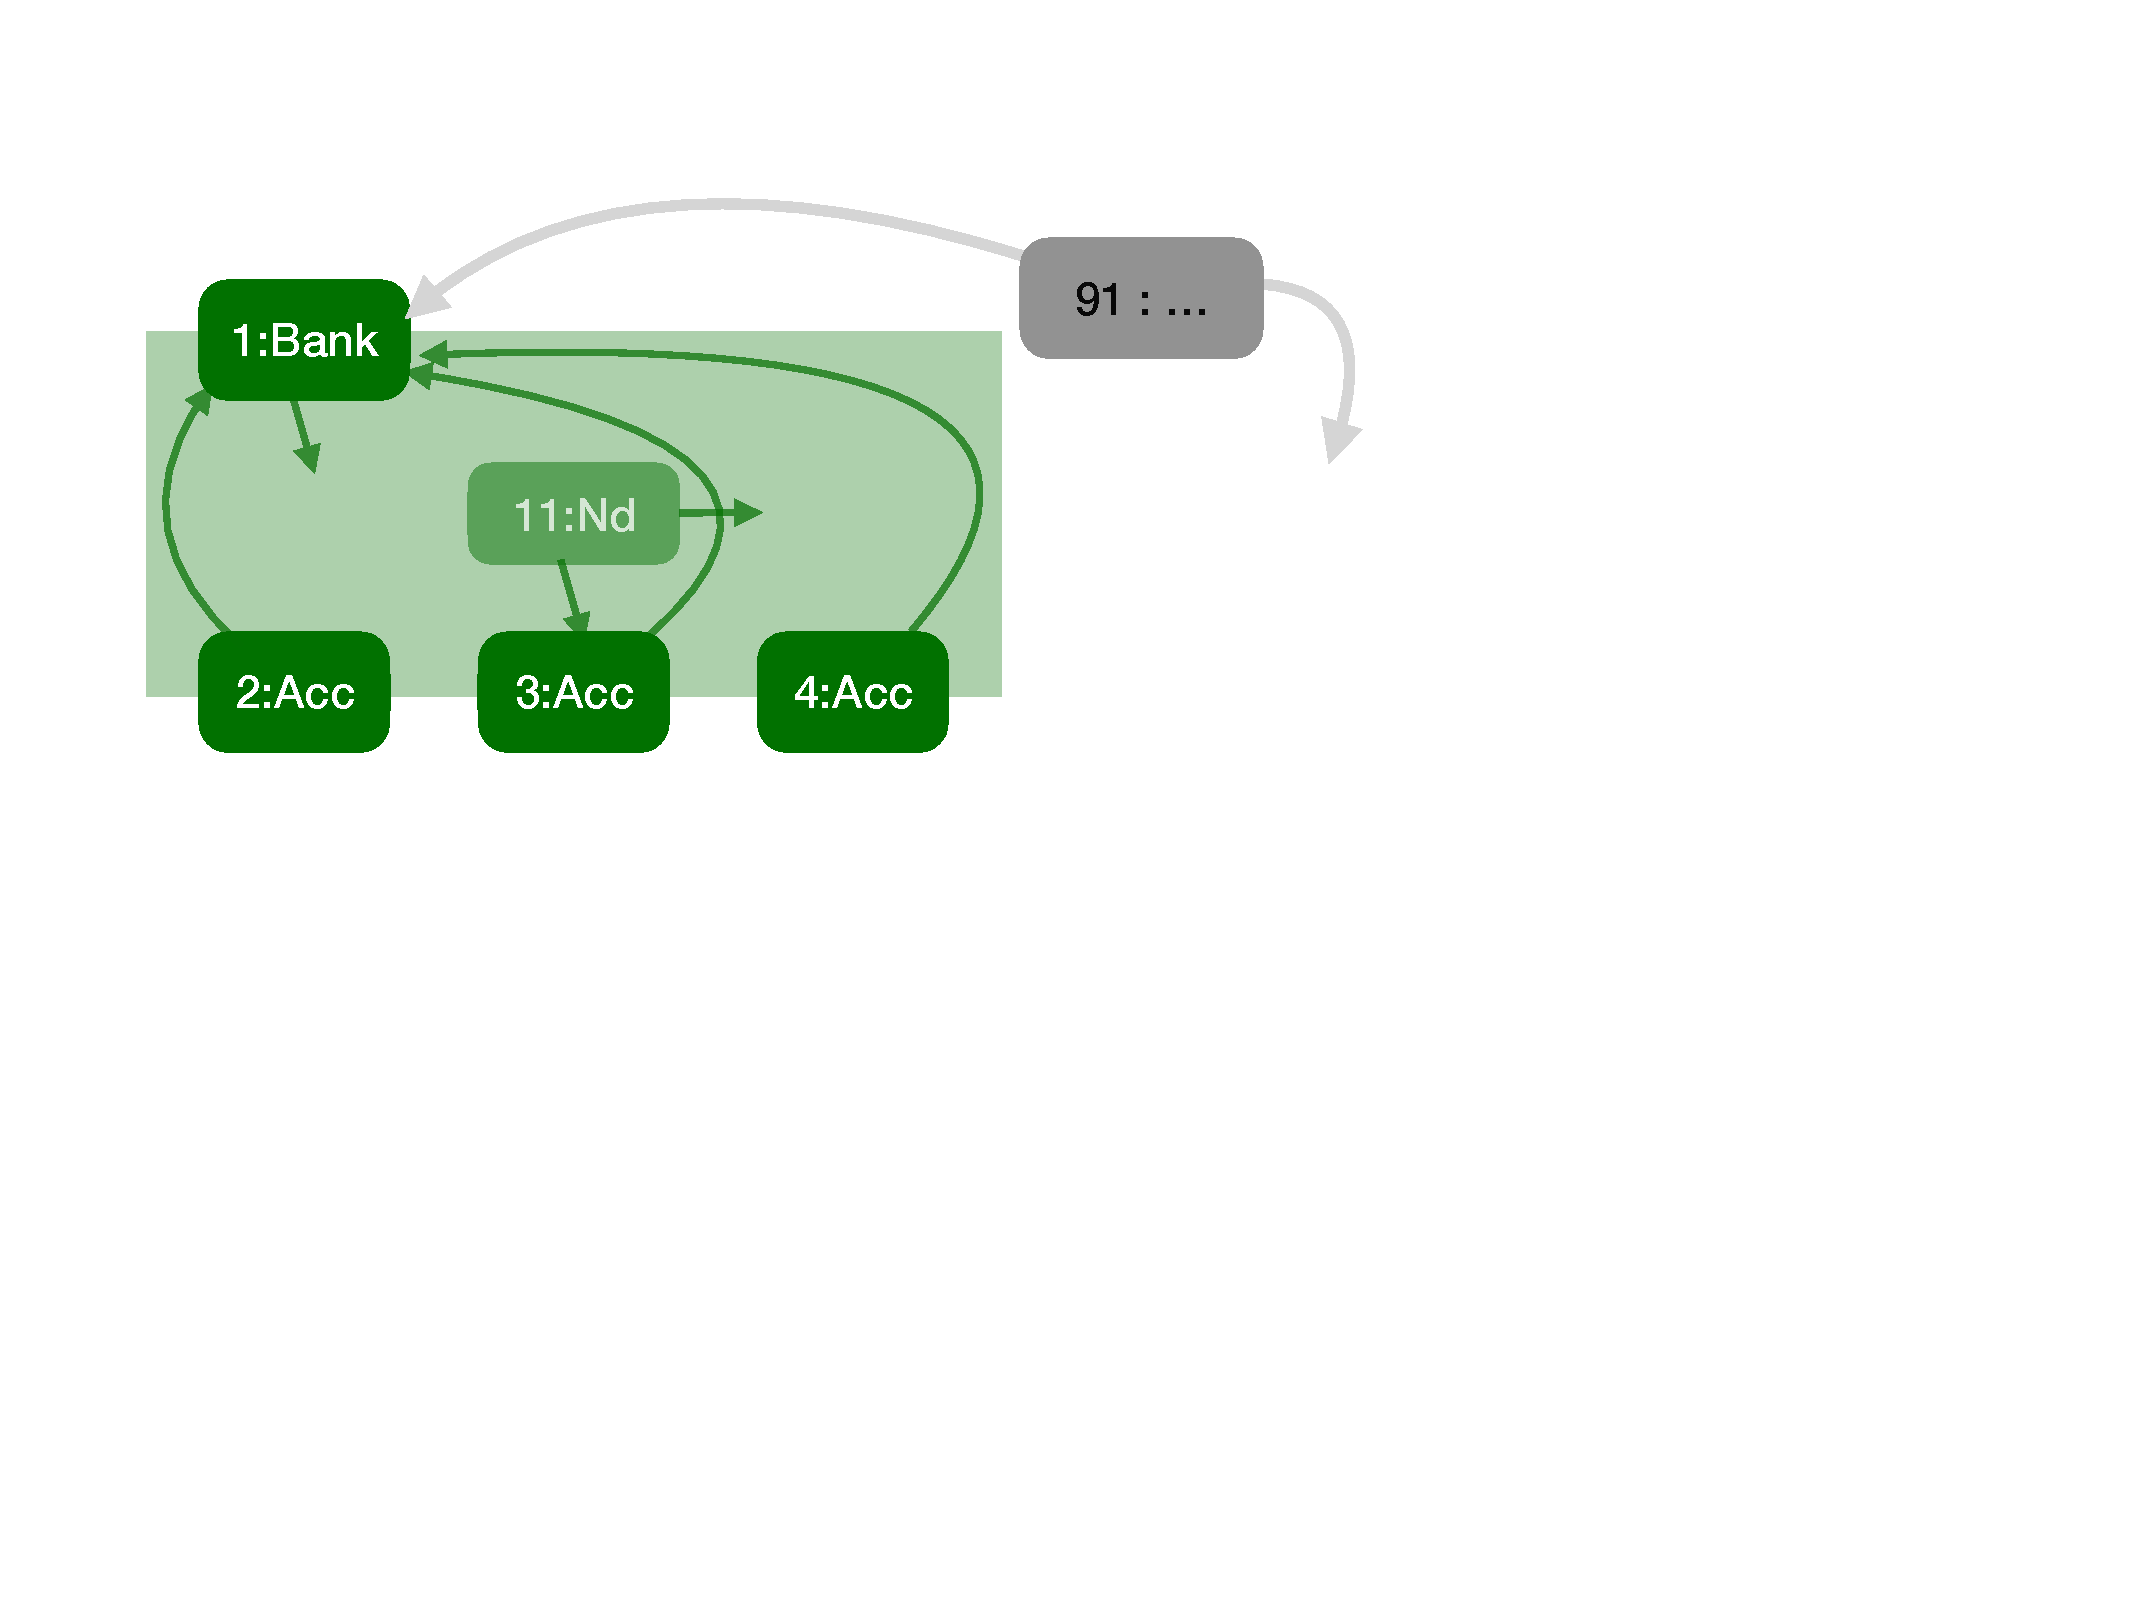
\includegraphics[width=\linewidth, trim=55  330 320 60,clip]{diagrams/BankAccount_version_2a.pdf}
   \end{minipage}
\end{tabular}
 
\sd{Note in the diagram above the dangling pointers at objects $1$,  $11$, and $91$ - reminiscent of the separation
of heaps into disjoint subheaps, as provided by the 
$*$ operator in separation logic \cite{Reynolds02}. The difference is that in separation logic, the 
separation is provided through the assertions, where $\A * \A'$ holds in any heap  which can be split into
disjoint $\chi$ and $\chi'$ where $\chi$ satisfies $\A$ and $\chi'$ satisfies $\A'$. That is, in $\A * \A'$  the split of the 
heap is determined by the assertions   $\A$ and $\A'$ and there is an implicit requirement of disjointness, while in $\restrct {\sigma}{\prg{S}}$ the split is
determined by \SF, and no disjointness is required.
}

We now define the semantics of $\Using {\A} {\prg{S}}$.


\begin{definition}[Space]  \label{def:valid:assertion:space} 
For any modules $\M$, $\M'$, assertions $\A$ and variable \prg{S}, we define$:$
\begin{itemize}
\item
 $\M\mkpair \M', \sigma \models \Using {\A} {\prg{S}}$
 \IFF
 $\M\mkpair \M', \restrct \sigma {\prg{S}} \models  \A  $.
\end{itemize}
\end{definition}
\jm{
\begin{definition}[Space]  \label{def:valid:assertion:space} 
For any modules $\M$, $\M'$, assertions $\A$ and variable \prg{S}, we define$:$
\begin{itemize}
\item
 $\M\mkpair \M', \sigma_0 \ldots \sigma \models \Using {\A} {\prg{S}}$
 \IFF
 $\M\mkpair \M', \restrct \sigma {\prg{S}} \models  \A  $.
\end{itemize}
\end{definition}
 }

\sd{
The set \SF\ in the assertion $\Using {\A} {\prg{S}}$ is related to  framing  from implicit dynamic frames \cite{IDF}:
 in an implicit dynamic frames assertion  \ $\textbf{acc}\, \prg{x.f}  * \A$, the frame $\prg{x.f}$ prescribes which locations
 may be used to determine validity of $\A$.
The difference is that frames are sets of locations (pairs of address and field), while our \prg{S}-es are sets of addresses.
 More  importantly,   implicit dynamic frames assertions whose frames are not large enough are badly formed, 
 while in our work, such assertions
are allowed and may   hold %(\eg $\M_{BA2}\mkpair \M', \sigma  \models \Using {(\not(\exists n.\acc_2.\prg{balance}=n))} {\prg{S}_4}$),  
or not, \eg   %$\M_{BA2}\mkpair \M', \sigma   \models \exists n.\acc_2.\prg{balance}=n$, while 
 $\M_{BA2}\mkpair \M', \sigma  \models \neg\ \Using {(\exists n.\acc_2.\prg{balance}=n)} {\prg{S}_4}$.
} 
 
 

\subsection{Satisfaction of Assertions - Time}
\label{sect:time} 
\sd{To deal with time, we are faced with four challenges:  a) validity of assertions in the future or the past needs to be judged in the 
future configuration, but using the bindings from the current one, 
b) the current configuration needs to store the code being executed, so
as to be able to calculate future configurations, c) when considering the future, we do not want to observe 
configurations which go beyond the frame currently at the top of the stack, d) there is no "undo" operator to deterministically enumerate
all the previous configurations.}

\sd{\sophia{Consider  challenge  a)  in some more detail: the assertion
$\Future {\x.\f=\prg{3}}$  is satisfied in the \emph{current} configuration   $\sigma_1$,
 if in some {\em future} configuration $\sigma_2$, the field  \f\, of the object that is pointed at 
 by \x\, in the {\em current} configuration ($\sigma_1$) has the value \prg{3}, that is, if
$\interp{ \interp{\x}{\sigma_1}.f}{\sigma_2} = 3$,   even if
in that future configuration \x\ denotes a different object (i.e. if $\interp{\x}{\sigma_1}\neq \interp{\x}{\sigma_2}$).}}
\sd{
% To address a),    we store the continuation, \prg{cntn}, in each stack frame.
To address this, we define an  auxiliary concept:
the operator\ $\adapt$\,,   where}
 $\sigma_1 \adapt\, \sigma_2$ adapts the second configuration to the top frame's view of the former: 
 it returns a new configuration whose stack \sophia{comes from $\sigma_2$  but is augmented with the view from the  top frame} 
   from $\sigma_1$ and where the continuation   has been consistently renamed. This allows us to interpret expressions  in   
   $\sigma_2$ but with the variables bound according to   $\sigma_1$; \eg we can obtain that value 
   of \prg{x} in configuration  $\sigma_2$ even if \prg{x} was out of scope in $\sigma_2$.  
 % That is, $\Future {\x.\f=\prg{3}}$  is satisfied in $\sigma$, if there exists a $\sigma'$ in the future of $\sigma$ such that
% $\sigma'[\prg{z}\mapsto\interp \sigma
 



 \begin{definition}[Adaptation] %  of Runtime Configurations]  
  \label{def:config:adapt}
 For runtime configurations $\sigma_1$, $\sigma_2$.$:$
 $~ $ 
\sophia{
\begin{itemize}
\item
$\sigma_1 \adapt \sigma_2 \triangleq (\phi_3\cdot\psi_2,\chi_2)$  \IFF 
\begin{itemize}
\item
  $ \phi_3=(\, \prg{contn}_2[\prg{zs}_2  / \prg{zs}' ], 
  \varMap_2[\prg{zs}'\mapsto \varMap_2({\prg{zs}}_2)][\prg{zs}_1\mapsto \varMap_1({\prg{zs}_1})] \, ) $,\ \ \ 
 where
\item
$\sigma_1=(\phi_1\cdot\_,\_)$,\ \ \  $\sigma_2= (\phi_2\cdot\psi_2,\chi_2)$, \ \ \  
% %  \\ $\ \strut \ \ \hspace{1.45in} $
% \item 
$\phi_1$=$(\_,\varMap_1)$, \ \ \  $\phi_2$=$(\prg{contn}_2,\varMap_2)$, \ \ 
%  \\ $\ \strut \ \ \hspace{1.45in} $     % $\phi''$ such that
 and
\item
% $\ \strut \ \ \hspace{1.45in} $
$\prg{zs}_1$=$dom(\varMap_1)$,  \ \  \ $\prg{zs}_2$=$dom(\varMap_2)$,  \ \  \ and \ \ \
%  \\ $\ \strut \ \ \hspace{1.45in} $      
\item
$\prg{zs}'$ is a set  of variables with  the  same cardinality as $\prg{zs}_2$, and
% %  \\ $\ \strut \ \ \hspace{1.45in} $  
%\item  
all variables in
$\prg{zs}'$  are fresh in $\varMap_1$ and in $\varMap_2$.
\end{itemize}
\end{itemize}
}
\end{definition}

\sophia{That is, in the new frame $\phi_2$ from above, we keep the same continuation as from $\sigma_2$ but rename all
variables with fresh names $\prg{zs}'$,   and combine the variable map  $\beta_1$  from $\sigma_1$ 
with the variable map $\beta_2$ from $\sigma_2$  while avoiding names clashes through
 the renaming $[\prg{zs}'\mapsto \varMap_2(\prg{zs}_2)]$.}
The consistent renaming of the continuation allows the correct modelling of execution, as needed   for the semantics of  nested time assertions, as \eg in $\Future {\x.\f=\prg{3} \wedge \Future {\x.\f=\prg{5}}}$.


\sd{
Having addressed challenge a) we turn our attention to the remaining challenges: We address challenge b) by storing the remaining code to be executed in \prg{cntn} in each frame. 
We address challenge c) by only taking the top of the frame when considering future executions.
Finally, we address challenge d) by considering only configurations which arise from initial configurations, and 
which lead to the current configuration. 
}


\begin{definition}[Time Assertions]  \label{def:valid:assertion:time}
For any modules $\M$, $\M'$, and assertion  $\A$ we define
\mrr{I've switched this from $\phi \mapsto (\phi, \chi)$; it might be wrong but it seems to be what the definition should be}  
\begin{itemize}
% \item
% $\M\mkpair \M', \sigma \models   \Changes{\prg{e}}$  \IFF
% $\exists \sigma'.\, [\ \ \M\mkpair \M',\sigma \leadsto \sigma' \ \wedge \interp{e}{\sigma} \neq \interp{e}{\sigma\triangleleft \sigma'} \ \  ]$.
 \item
  $\M\mkpair \M', \sigma \models  \Next \A $
  \IFF
  $\exists \sigma'.\, [\ \ \M\mkpair \M',(\phi, \chi) \leadsto  \sigma' \ \wedge \M\mkpair \M',\sigma\adapt\sigma' \models \A \ \  ]$,
 \\
$\strut ~ \hspace{1.4in} $ \hfill  and where $\sigma$=$(\phi\cdot\_,\chi)$.\item
  $\M\mkpair \M', \sigma \models  \Future \A $
  \IFF
  $\exists \sigma'.\, [\ \ \M\mkpair \M',(\phi, \chi) \leadsto^* \sigma' \ \wedge \M\mkpair \M',\sigma\adapt\sigma' \models \A \ \  ]$,
 \\
$\strut ~ \hspace{1.4in} $   \hfill   and where $\sigma$=$(\phi\cdot\_,\chi)$.  
  \item
 $\M\mkpair \M', \sigma \models  \Prev \A $ \IFF
 $\forall \sigma_1, \sigma_2. [\ \ \Initial{\sigma_1}\ \wedge \   \M\mkpair \M', \sigma_1  \leadsto^*  \sigma_2 $\\
 $\strut ~ \hspace{2.1in}   \wedge \   \M\mkpair \M', \sigma_2  \leadsto   \sigma  
 \ \  \ \longrightarrow \ \ \   \
 \M\mkpair \M', \sigma\adapt\sigma_2  \models \A\ \
 ]$ 
 \item
 $\M\mkpair \M', \sigma \models  \Past \A $ \IFF
% $\forall \sigma_1, ... \sigma_n. [\ \ \Initial{\sigma_1}\ \wedge \  \sigma_n=\sigma $\\
% $\strut ~ \hspace{1.9in}   $   \hfill   $  \wedge \ \ \forall  i\in[1..n). \M\mkpair \M', \sigma_{i} \leadsto  \sigma_{i+1}$
% $\strut ~ \hspace{1.9in} $   \hfill   $ \longrightarrow \ \ \ ( \  \exists j\in [1..n-1).
% \M\mkpair \M', \sigma\adapt\sigma_j  \models \A\ \
%
$\forall \sigma_1. [\ \ \Initial{\sigma_1}\ \wedge \  \M\mkpair \M',\sigma_1 \leadsto^* \sigma \longrightarrow $\\
 $\strut ~ \hspace{0.1in} $   \hfill   $(\ \  \exists \sigma_2.
 \M\mkpair \M',\sigma_1 \leadsto^* \sigma_2 \ \wedge\  \M\mkpair \M',\sigma_2 \leadsto^* \sigma \ \wedge \ 
 \M\mkpair \M', \sigma\adapt\sigma_2  \models \A\ \ 
 )]$ 
\end{itemize}
\end{definition}
\jm{
\begin{definition}[Constrained Reduction]  \label{def:constrained_reduction}
For any modules $\M$, $\M'$, and configurations $\sigma_1$, $\sigma_2$\\
\begin{itemize}
\item
$\M\mkpair \M',  \sigma_1\lceil\leadsto\rceil \sigma_2$ 
\IFF
$\M\mkpair \M',  (\phi \cdot \_, \chi_1) \leadsto(\psi, \chi_2)$\\
$\strut ~ \hspace{1.4in} $ \hfill 
where
$\sigma_1 = (\phi \cdot \psi_1, \chi_1)$ and $\sigma_2 = (\psi \cdot \psi_1, \chi_2)$
and
\item
$\M\mkpair \M',  \sigma_1\lceil\leadsto^*\rceil \sigma_2$ 
\IFF
$\M\mkpair \M',  (\phi \cdot \_, \chi_1) \leadsto^* (\psi, \chi_2)$\\
$\strut ~ \hspace{1.4in} $ \hfill 
where
$\sigma_1 = (\phi \cdot \psi_1, \chi_1)$ and $\sigma_2 = (\psi \cdot \psi_1, \chi_2)$
\end{itemize}
\end{definition}
\begin{definition}[Time Assertions]  \label{def:valid:assertion:time}
For any modules $\M$, $\M'$, and assertion  $\A$ we define
\begin{itemize}
% \item
% $\M\mkpair \M', \sigma \models   \Changes{\prg{e}}$  \IFF
% $\exists \sigma'.\, [\ \ \M\mkpair \M',\sigma \leadsto \sigma' \ \wedge \interp{e}{\sigma} \neq \interp{e}{\sigma\triangleleft \sigma'} \ \  ]$.
 \item
  $\M\mkpair \M', \sigma_0 \ldots \sigma \models  \Next \A $
  \IFF
  $\exists \sigma'.\, [\ \ \M\mkpair \M',\sigma \lceil\leadsto\rceil \sigma' \ \wedge \M\mkpair \M',\sigma_0 \ldots \sigma \models \A \ \  ]$
  \item
  $\M\mkpair \M', \sigma_0 \ldots \sigma \models  \Future \A $
  \IFF
  $\exists \sigma'.\, [\ \ \M\mkpair \M',\sigma \lceil\leadsto^*\rceil \sigma' \ \wedge \M\mkpair \M',\sigma_0 \ldots \sigma \models \A \ \  ]$
  \item
 $\M\mkpair \M', \sigma_0 \ldots \sigma \models  \Prev \A $ \IFF
$\forall \sigma'. [\ \  \M\mkpair \M',\sigma_0 \leadsto^* \sigma' \wedge \M\mkpair \M',\sigma' \leadsto \sigma \longrightarrow $\\
 $\strut ~ \hspace{0.1in} $   \hfill 
$ \M\mkpair \M', \sigma_0 \ldots \sigma'  \models \A\ \ 
 ]$ 
 \item
 $\M\mkpair \M',\sigma_0 \ldots  \sigma \models  \Past \A $ \IFF
$\forall \sigma'. [\ \  \M\mkpair \M',\sigma_0 \leadsto^* \sigma' \wedge \M\mkpair \M',\sigma' \leadsto^* \sigma \longrightarrow $\\
 $\strut ~ \hspace{0.1in} $   \hfill   
 $\M\mkpair \M', \sigma_0 \ldots \sigma'  \models \A\ \ 
 ]$ 
\end{itemize}
\end{definition}
}

%Thus,  $\M\mkpair \M', \sigma \models  \Future \A $ holds if
%$\A$ holds in some configuration $\sigma'$ which arises from execution of $\phi$, where $\phi$ is the top frame of $\sigma$. By requiring that $\phi \leadsto^* \sigma' $ rather than
%$\sigma \leadsto^* \sigma' $ we are restricting the set of possible future configurations to
%just those that are caused by the top frame;
%that is, we do not want to consider the effect of  enclosing function calls.
%
%This allows us to write more natural specifications
%when giving necessary conditions for some future effect.
 
 In general, $\Using {\Future {\A}} {\SF}$ is different from
  $\Future {\Using {\A} {\SF}}$. In the former assertion, $\SF$ must contain
   every extant object involved in reaching the future configuration\mrr{Originally read ``\textsc{as well as the objects needed to
    then establish validity of $\A$ in that future configuration}''  No it doesn't, this is wrong. It need only have the objects that are needed in creating that future. This means that objects in $\SF$, plus the objects created by the reduction, are used in A}, whilst in the latter, 
     $\SF$ needs instead to contain the objects needed to establish $\A$ in that future configuration.
    % chopped as the example no longer works.
  For example, revisit Fig. \ref{fig:BankAccountDiagrams}, and take $\SF_1$ to consist of objects \prg{1}, \prg{2},   \prg{4}, \prg{93}, and \prg{94},
  and $\SF_2$ to consist of objects \prg{1}, \prg{2},   \prg{4}.  Assume that 
   $\sigma_5$ is like $\sigma_1$, that the next call in $\sigma_5$ is a method on $\prg{u}_{94}$, whose  body obtains the
  address of $\acc_4$ (by making a call on \prg{93} to which it has access), and the address of $\acc_2$ (to which it has access),
  and then makes the call $\acc_2.\prg{deposit}(\acc_4,360)$. Assume also     that $\prg{a}_4$'s balance is \prg{380}.
  %Assume   that $\sigma_1$ contains the
  % call $\prg{m()}$ with receiver $\pu_{94}$ and that the code of \prg{m} and \prg{m2} is as above. 
  Then\\
  $\strut$ \hspace{1.1cm}  $\M_{BA1}\mkpair ..., \sigma_5 \ \models \ \Using {\Future{ \Changes {\acc_2.\bal}}} {\SF_1}$\\
   $\strut$ \hspace{1.1cm}  $\M_{BA1}\mkpair ..., \sigma_5 \ \not\models \ \Using {\Future{ \Changes {\acc_2.\bal}}} {\SF_2}$\\
 $\strut$ \hspace{1.1cm}  $\M_{BA1}\mkpair ..., \sigma_5 \ \models \ \Future{ \Using {\Changes {\acc_2.\bal}} {\SF_2}}$\

Whilst the above shows that from $\Future { \Using{A}{\SF} }$ we cannot conclude $\Using { \Future{A} }{\SF}$, it is also worth noting that in general the inverse doesn't hold either. $\Future { \Using{A}{\SF} }$ restricts $A$ in the future, meaning any objects instantiated in the between the present and then are excluded, whereas $\Using { \Future{A} }{\SF}$ restricts the space in the present, so the objects are considered in A. Taking a new configuration $\sigma_6$  with continuation \prg{x := new Account(100, null) } and otherwise similar to $\sigma_1$, and $\SF = \emptyset$, we cannot prove $\M_{BA1}\mkpair ..., \sigma_6 \ \models \ \Future{ \Using { \prg{x.bank} = \prg{null} } {\SF}}$  as \prg{x} is not in $S$, however, we can prove $\M_{BA1}\mkpair ..., \sigma_6 \ \models \ \Using { \Future{ \prg{x.bank} = \prg{null} } } {\SF}$, since the restriction of the configuration to $\SF$ in the present doesn't prevent the next statement's new \prg{Account} being considered in the \Future{\cdot}.


\subsection{Properties of Assertions}

 
\label{sect:classical} 
We define equivalence of   assertions in the usual way: assertions $\A$ and $\A'$are equivalent if they are satisfied  in
the context of the same configurations and module pairs -- \ie\\
 \strut \hspace{1.1cm} $\A \equiv \A'\  \IFF\    \forall \sigma.\, \forall \M, \M'. \ [\ \ \M\mkpair \M', \sigma \models \A\ \mbox{ if and only if }\ \M\mkpair \M', \sigma \models \A'\ \ ].$\\
We can then prove that the usual equivalences hold, \eg\  $ \A \vee \A' \ \equiv \  \A' \vee \A$, and\   $\neg (\exists \prg{x}.\A )  \  \ \equiv \  \forall \prg{x}.(\neg  \A)$.
%
Our assertions are classical, \eg  $ \A \wedge\neg \A \ \equiv \  \prg{false}$, and $\M\mkpair \M', \sigma  \models \A$ and  $\M\mkpair \M', \sigma  \models \A \rightarrow \A'$  implies
$\M\mkpair \M', \sigma  \models \A '$. 
 \sd{This desirable property comes at the loss of some expected equivalences, \eg, in general, 
 $\e = \prg{false}$ and $\neg\e$ are not equivalent. 
 More  in Appendix \ref{app:assertions}.}

\subsection{Modules satisfying assertions}

Finally, we define satisfaction of assertions by modules: a module
$\M$ satisfies an assertion $\A$ if for all other potential modules $\M'$, in all configurations arising from executions of $\M\mkpair\M'$, the assertion $\A$ holds.

\begin{definition}
\label{def:module_satisfies}
For any module $\M$, and  assertion $\A$, we define:
\begin{itemize}
\item
$\M \models \A$ \IFF  $\forall \M'.\, \forall \sigma_0, \Initial{\sigma_0}, \ \sigma\!\in\!\Arising{\M\mkpair\M', \sigma_0}.\   \M\mkpair\M', \sigma_0 \ldots \sigma \models \A$
\end{itemize}
\end{definition}

 




